\documentclass{article}
\usepackage[T1,T2A]{fontenc}
\usepackage[utf8]{inputenc}
\usepackage[english,ukrainian]{babel}
\usepackage[]{amsthm} %lets us use \begin{proof}
\usepackage[]{amssymb} %gives us the character \varnothing
\usepackage{graphicx}

\begin{document}

\title{Семінар 15. Ізоморфізм графів}
\date{19 червня 2023}

\maketitle

\begin{figure}[ht!]
\centering
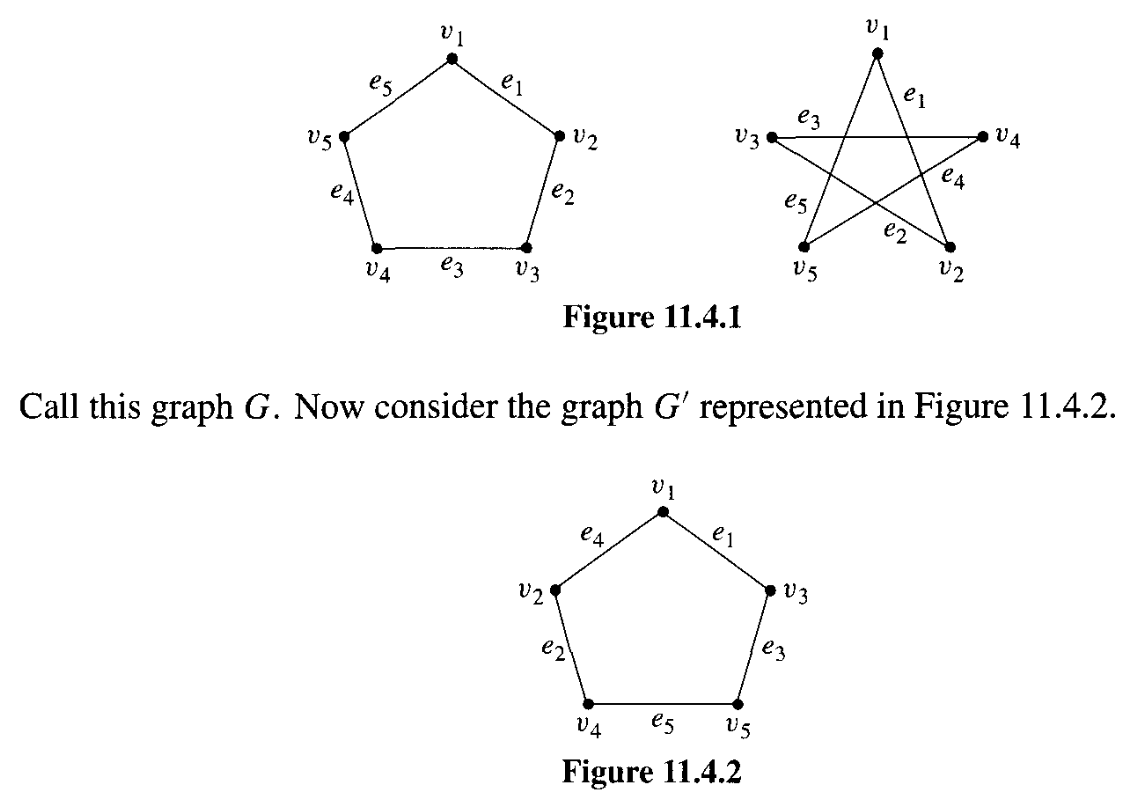
\includegraphics[width=90mm]{1}
\end{figure}

\begin{figure}
\centering
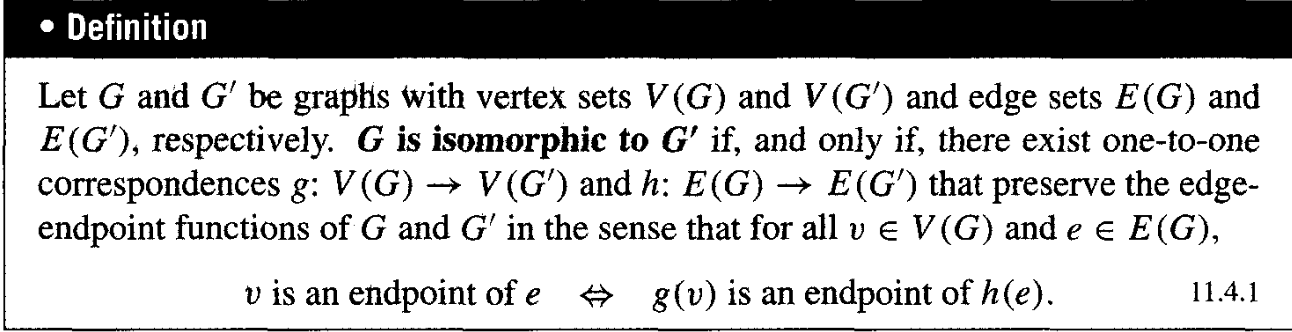
\includegraphics[width=90mm]{2}
\end{figure}

\begin{figure}
\centering
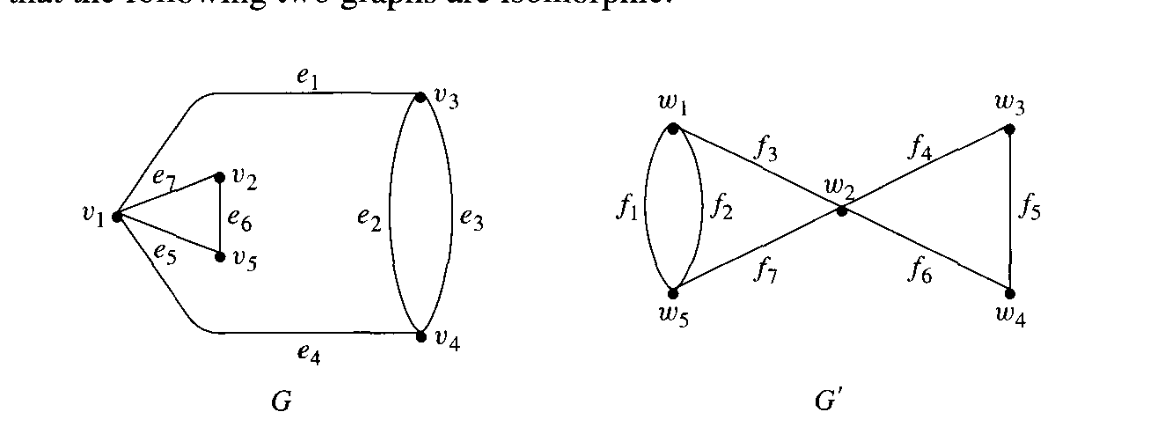
\includegraphics[width=90mm]{3}
\end{figure}

\begin{figure}
\centering
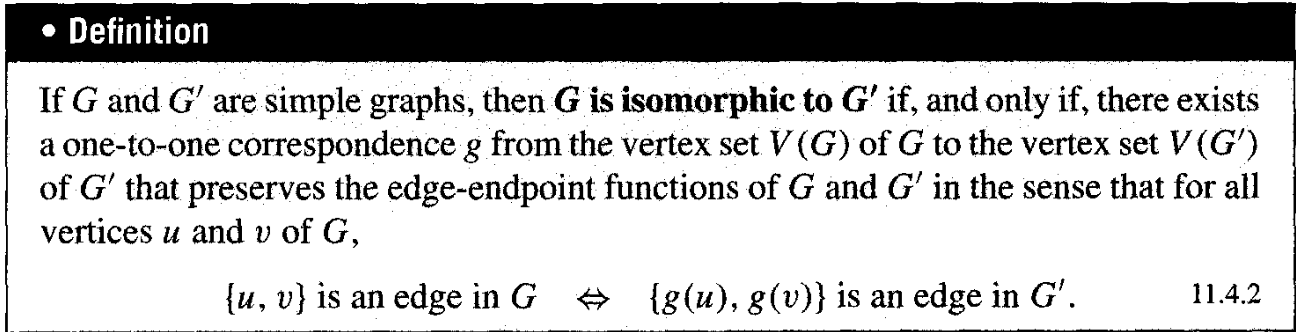
\includegraphics[width=90mm]{4}
\end{figure}

\begin{figure}
\centering
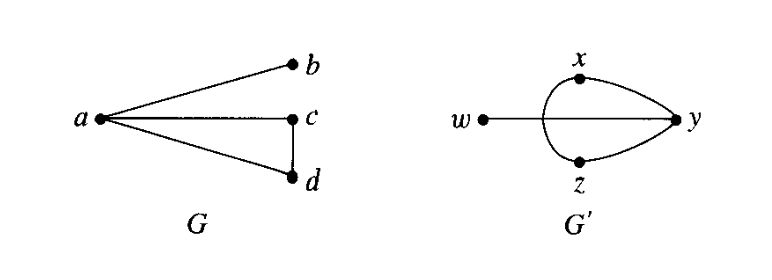
\includegraphics[width=90mm]{5}
\end{figure}

\begin{figure}
\centering
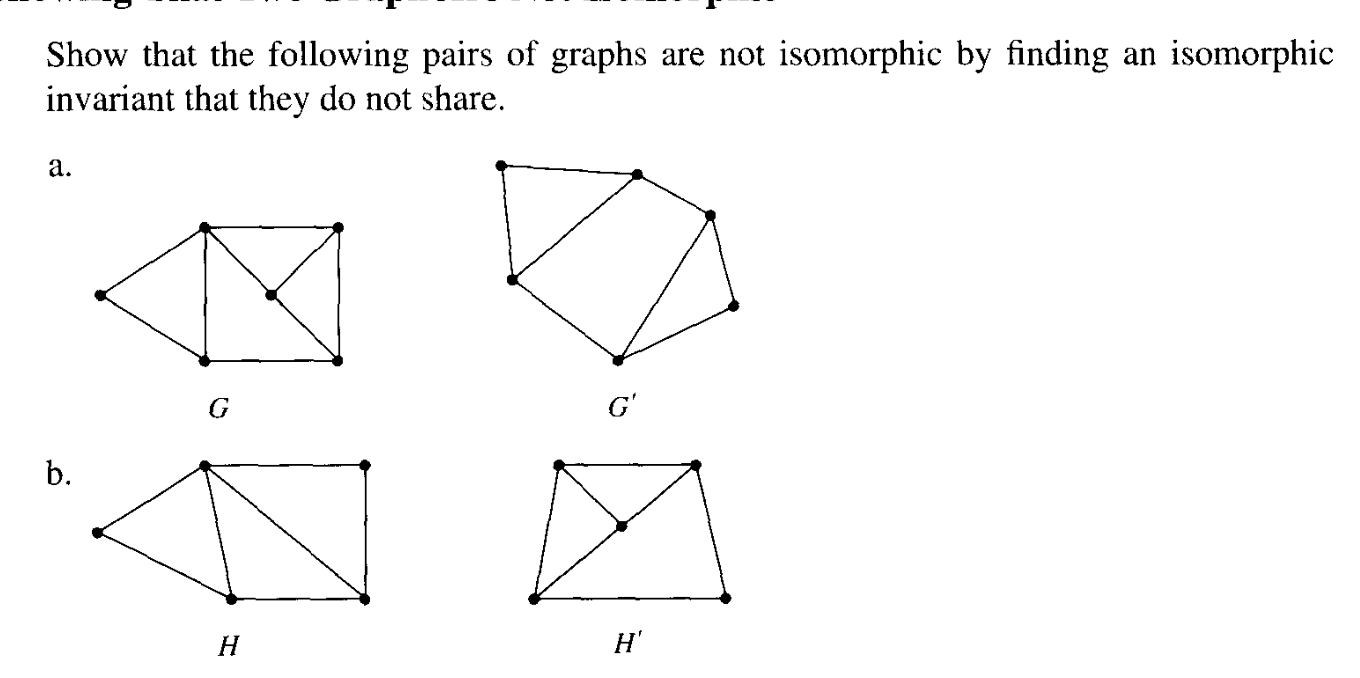
\includegraphics[width=90mm]{7}
\end{figure}

\begin{figure}
\centering
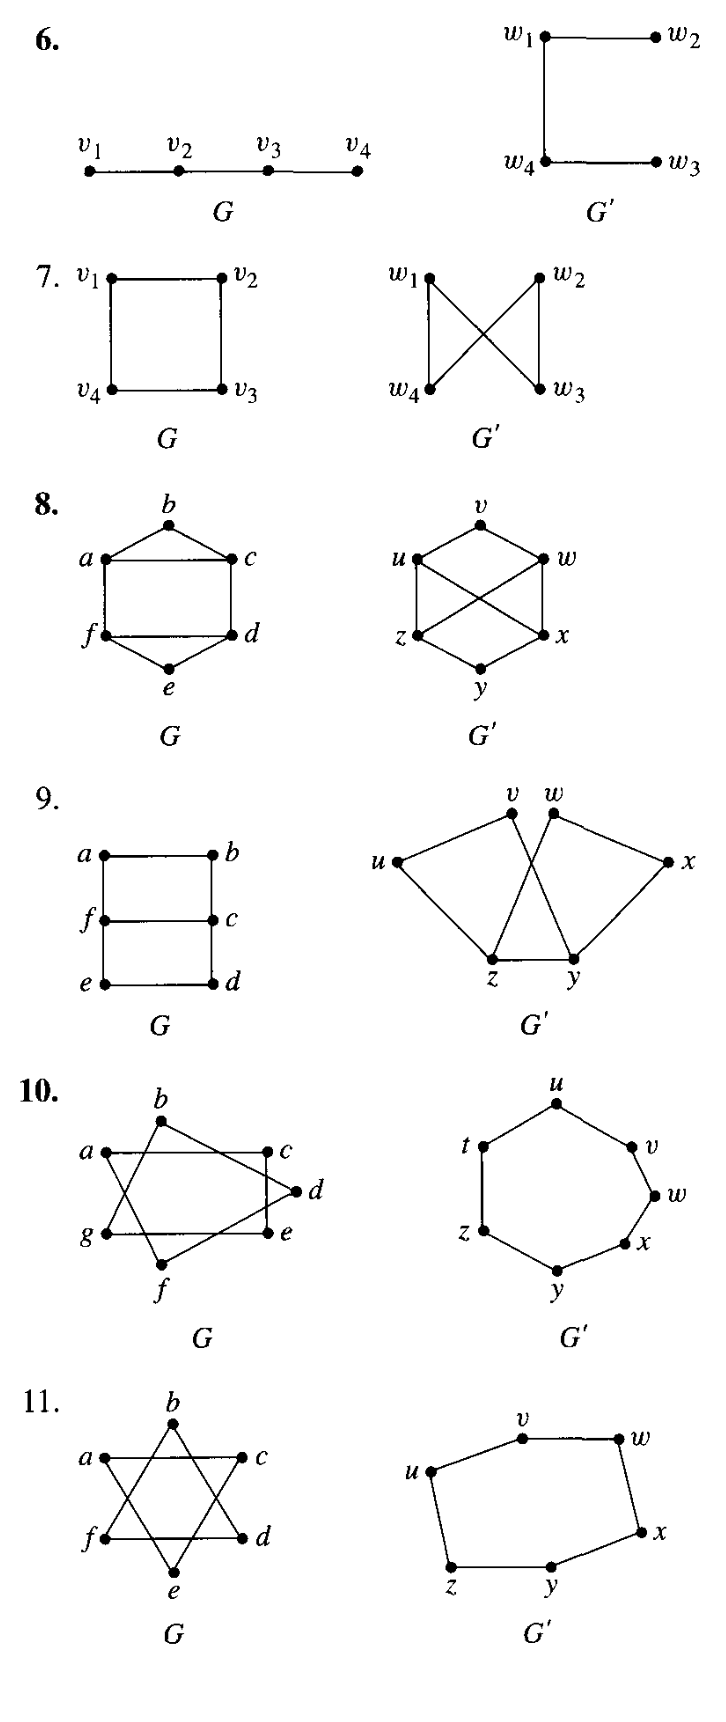
\includegraphics[width=90mm]{8}
\end{figure}

\begin{figure}
\centering
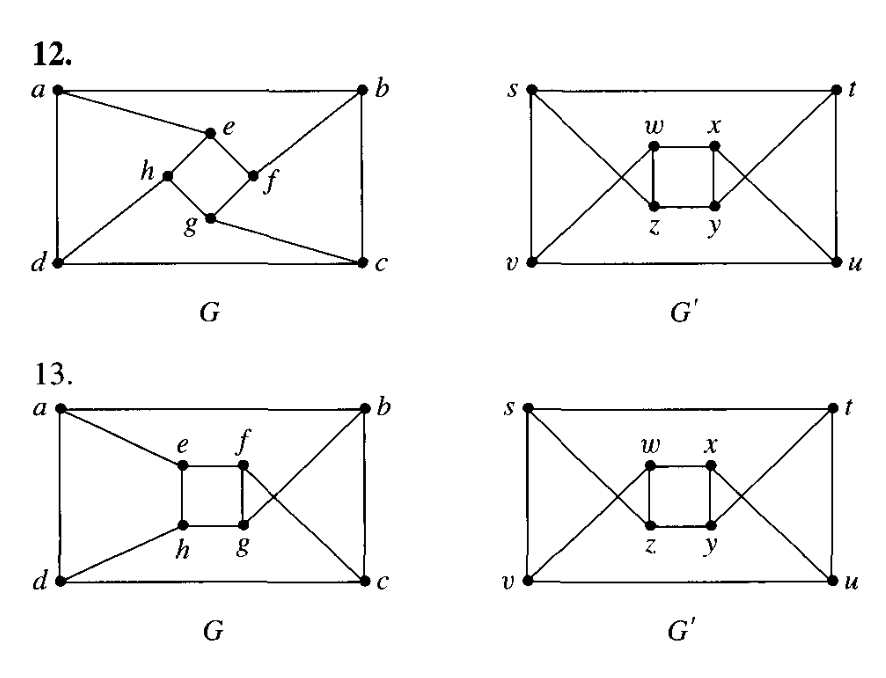
\includegraphics[width=90mm]{9}
\end{figure}

\begin{figure}
\centering
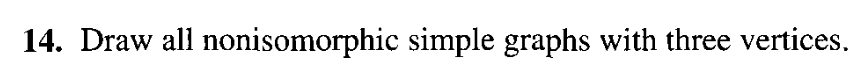
\includegraphics[width=90mm]{10}
\end{figure}

\end{document}